% 4-6 pages total.

% Goals:
% Analysis (~2-3 pages).
% Discuss the background (1 page).
% Clearly explain the problem. Specify the aims and objectives - ordered list of features and justification (~2 pages).

% Explain how the requirements are gathered (the tools and techniques used) (1/2 page to 1 page).
% Consider applying SMART crieria to requirements (https://www.win.tue.nl/~wstomv/edu/2ip30/references/smart-requirements.pdf):
	% Specific
	% Measurable
	% Attainable
	% Realisable
	% Traceable
% User stories and MOSCOW statements in the Appendix.

% Marking:
% Has the student surveyed relevant literature and existing software products? Has he captured the requirements? Has he analysed the problem, and devised a suitable approach for solving the problem?
% A-band: The problem analysis is excellent. The survey is comprehensive. The approach is clearly feasible and innovative.

\chapter{Analysis \& Requirements}\label{analysis_requirements}

\section{Background}

A two-dimensional image has the power to communicate complex multi-dimensional information about its subject.
An accurate depiction may convey a subject's form, texture, and depth relationship to other objects, which in turn allows us to intuitively build a mental model of a scene.

For this to be achieved effectively, the style in which an image is produced must be selected appropriately based upon the communicational goals of the artist.
For example, a traditional landscape watercolourist, technical writer, or marketeer all may wish to convey information about a given subject - all however will have substantially different goals.

This disjoint in user requirements is particularly interesting when it comes to production of computer generated graphics, of which the majority of development has focussed upon producing photorealistic images.
Photorealism may be perfect for the automotive marketeer who wishes to present car designs to the public, however such an approach is less well-suited to the technical manuals of the same car, where the goal is to accurately convey fit, form and function of mechanical parts.
Indeed, the medium upon which the image is to be delivered also plays an important role.
For example, a high-resolution, full-colour, photorealistic image may be appropriate for a magazine. 
A more abstract representation of the same parts may better convey the details required of the monochrome technical manual, where knowledge of surface texture and glossiness at best fail to add value, at worst may even distract the reader.

Indeed, such non-photorealistic techniques have historically been used to great effect in technical disciplines such as engineering \citep{porter1988} and mathematics \citep{francis2007}, where precise communication of the specificities of structure is paramount. Styles can also be tailored to suit less obvious needs - for example, compared to photorealism, bolder styles can have benefits in terms of reduced degradation of image detail when subject to multiple stages of reproduction. Subtler styles can be applied to achieve effective results with very limited use of colour and ink, leading to improved economy for high-volume printing.

\begin{figure}[h]
	\centering
	\begin{subfigure}[b]{0.3\textwidth}
		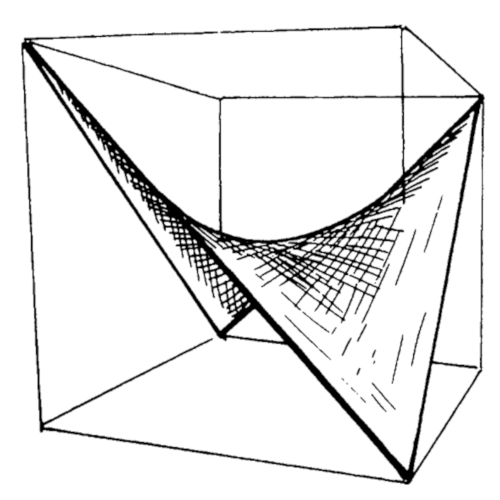
\includegraphics[height=3.5cm]{images/ex_hand_drawn1}
		\caption{Mathematical surface, rendered with hatches and a bounding box to convey depth information.}\label{ex_hand_drawn1}
	\end{subfigure}
	\begin{subfigure}[b]{0.3\textwidth}
		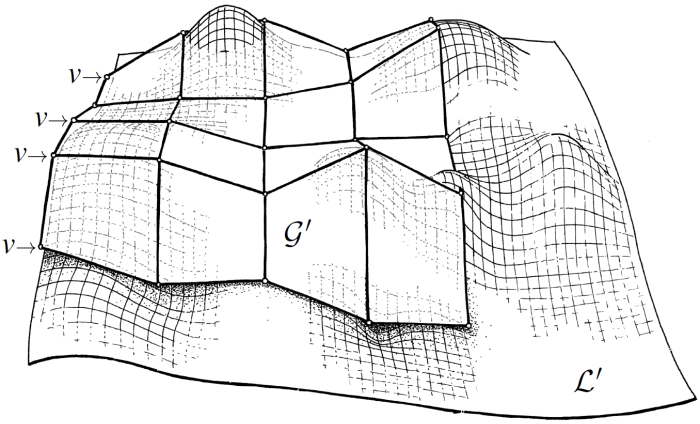
\includegraphics[width=4.5cm]{images/ex_hand_drawn2}
		\caption{Surface plot, rendered with streamlines depicting surface curvature.}\label{ex_hand_drawn2}
	\end{subfigure}
	\begin{subfigure}[b]{0.3\textwidth}
		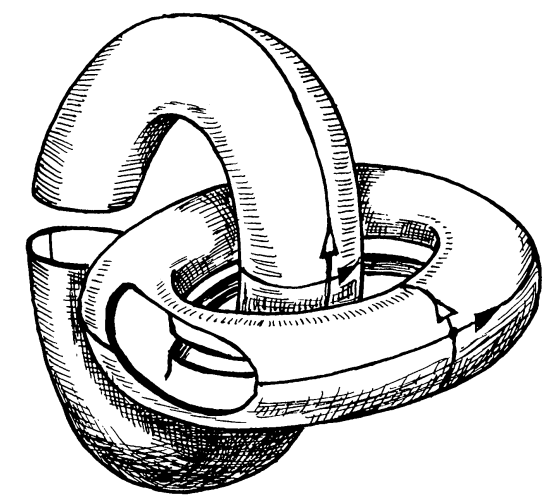
\includegraphics[height=3.5cm]{images/ex_hand_drawn3}
		\caption{Cross-hatching used to convey form and lighting.}\label{ex_hand_drawn3}
	\end{subfigure}
	\caption{Traditional hand-drawn technical renderings.}
\end{figure}

The aim of the field of Non-Photorealistic Rendering (NPR) is to produce computer-generated images based upon such principles of traditional or digital art.
Styles attainable through NPR techniques are many and varied, and include painting techniques such as watercolour, oils and pointillism; pen-and-ink techniques such as stippling and cross-hatching; and 3D shading techniques such as cel-shading.
Styles themselves may be manipulated by the artist to add expression - focusing the viewer's attention to areas of particular importance, whilst abstracting away unnecessary detail.
As such, compared to photorealism, traditional techniques realised through NPR allow certain classes of visual information to be effectively conveyed in-line with the communicational goals of the artist.

\section{State of the Art}

The previous section speaks to the benefit traditional drawing styles can bring to precisely communicate visual information. Unfortunately, actual implementation of NPR techniques in today's popular, widely available and easy to use rendering engines is limited, and often tailored to cartoon/anime styles (cel, Gooch shading).
There is generally poor support for technical monochrome styles such as hatching, which is surprising given the strong tradition of such styles in technical disciplines.

The NPR sub-field of Stroke Based Rendering (SBR) presents some interesting techniques to address computer-aided implementation of traditional techniques.
An excellent paper by Aaron Hertzmann \citep{hertzmann2002} summarises a selection of SBR approaches to automatically (or semi-automatically) create images by placing discrete strokes, based on some direction from the user.

Hertzmann reports that some techniques - such as Haeberli's painterly algorithm \citep{haeberli1990} - have been adopted into commercial drawing applications, however even as of today (2018) implementation of technical pen-and-ink styles do not appear to be as accessible. As such an opportunity is identified to close this gap.

\section{Chosen Platform}

Blender\footnote{\url{https://www.blender.org}} is a software package with capability for 2D sketching, 3D modelling, animation, physics simulation and rendering.
Licensed under the GNU General Public License, Blender is free to use and as such enjoys widespread adoption across multiple fields.
The software ships with a selection of rendering engines which can be used to produce high-quality output.

The most prominent example, Cycles\footnote{\url{https://www.cycles-renderer.org}}, is a physically-based, path-tracing rendering engine which aims to accurately simulate the interaction of light with various kinds of materials.
This makes Cycles well-suited for producing photorealistic renderings (Figure \ref{ex_photoreal}).
A limited range of NPR styles are feasible with Cycles, however these are mostly suited to non-technical styles (Figures \ref{ex_toon1}, \ref{ex_toon2}).

\begin{figure}[h]
	\centering
	\begin{subfigure}[b]{0.3\textwidth}
		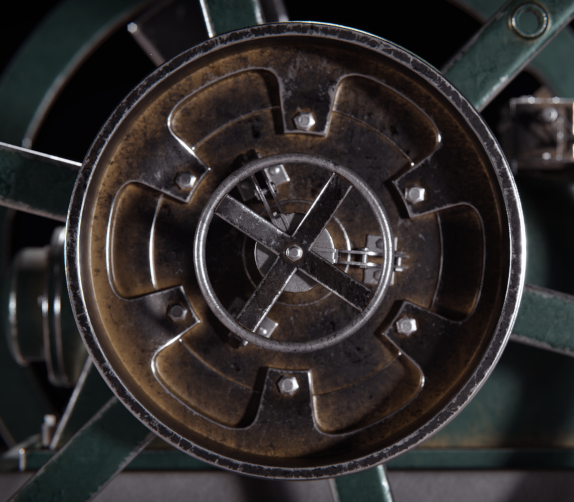
\includegraphics[height=3.25cm]{images/ex_photoreal}
		\caption{Photorealistic rendering, showing accurate light transport and material modelling.}\label{ex_photoreal}
	\end{subfigure}
	\begin{subfigure}[b]{0.3\textwidth}
		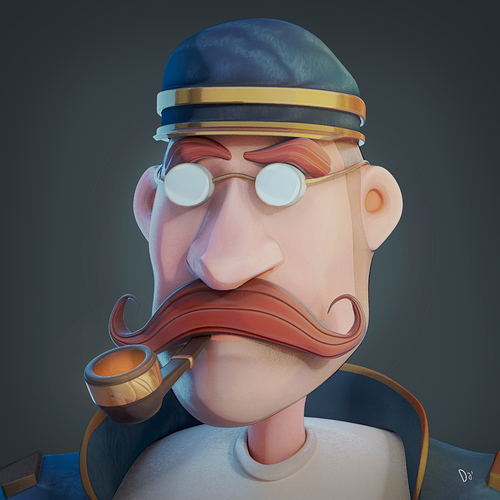
\includegraphics[height=3.25cm]{images/ex_toon1}
		\caption{Stylised rendering, accurate lighting with artificial materials.}\label{ex_toon1}
	\end{subfigure}
	\begin{subfigure}[b]{0.3\textwidth}
		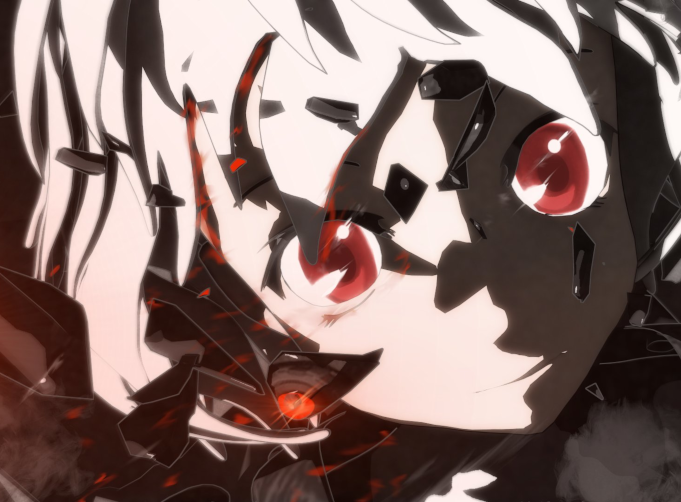
\includegraphics[height=3.25cm]{images/ex_toon2}
		\caption{Cel-shading rendering, limited use of shading in favour of stark boundaries of colour.}\label{ex_toon2}
	\end{subfigure}
	\caption{Cycles renderings.}
\end{figure}

The Freestyle\footnote{\url{http://freestyle.sourceforge.net}} edge-and-line-based NPR engine has shipped with Blender as of version 2.67. This engine allows for a wider range of sketchy (Figures \ref{ex_sketchy1}, \ref{ex_sketchy2}) and technical (Figure \ref{ex_line}) styles. However, a limitation of Freestyle is the inability to place strokes on faces, which leaves many NPR shading styles out of reach. This greatly limits the ability of Freestyle to effectively communicate surface details through traditional techniques.

\begin{figure}[h]
	\centering
	\begin{subfigure}[b]{0.3\textwidth}
		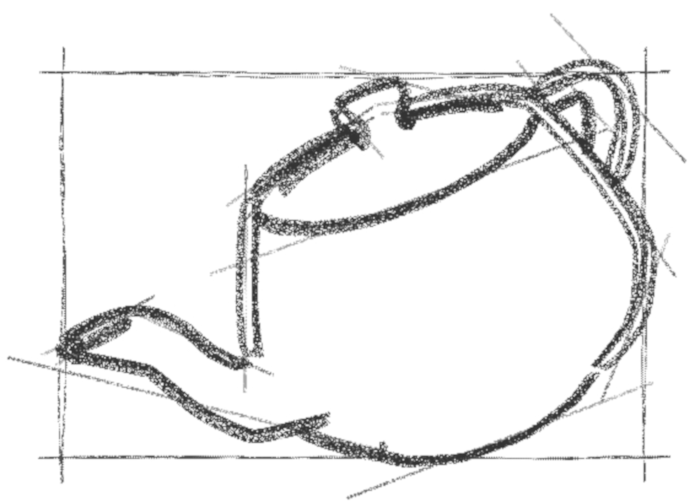
\includegraphics[height=3.25cm]{images/ex_sketchy1}
		\caption{Charcoal line styles, rough sketch style.}\label{ex_sketchy1}
	\end{subfigure}
	\begin{subfigure}[b]{0.3\textwidth}
		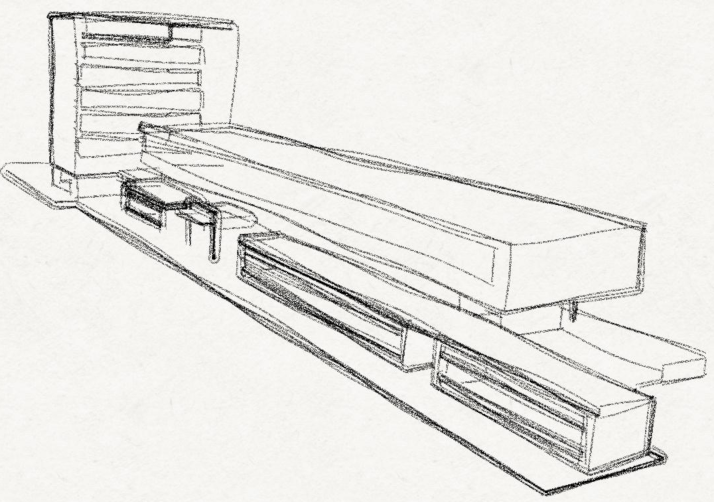
\includegraphics[height=3.25cm]{images/ex_sketchy2}
		\caption{Pencil perspective, rough sketch style.}\label{ex_sketchy2}
	\end{subfigure}
	\begin{subfigure}[b]{0.3\textwidth}
		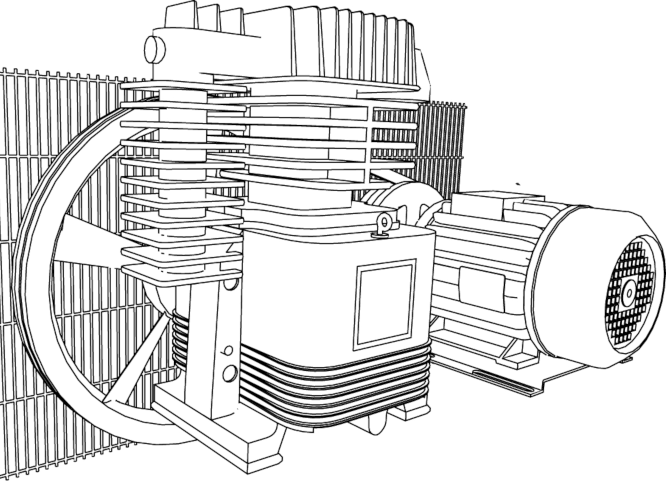
\includegraphics[height=3.25cm]{images/ex_line}
		\caption{Simple line perspective, technical style.}\label{ex_line}
	\end{subfigure}
	\caption{Freestyle renderings.}
\end{figure}

\section{Problem Definition}

A project was undertaken to extend Blender by developing an add-on (plug-in) written in Python (hereinafter the ``System''). The aim of the System is to allow the user to automatically produce high-quality renders of traditional, hand-drawn appearance, through application of traditional monochrome drawing techniques.

Although the System is automated, control is afforded to the User, allowing specification of subtle or bold styles, which are tailored for expressing structure, using minimal quantities of ink.

System scope is limited to communication of mathematical surfaces. The primary use-case is creation of images for publication in technical papers or lecture slides/notes.

The Customer and primary user is identified as John H Williamson, Lecturer, School of Computing Science, University of Glasgow.

\section{Planning}

Based upon the initial project brief\footnote{\url{https://github.com/cjbel/blender-hand-drawn-npr/wiki/Project-Brief}}, the approach taken was to stake-out all required high-level tasks and assign sensible durations to outline a feasible path. 
In order to have meaningful discussions regarding detailed requirements (and reasonable gut-feel for levels of feature feasibility), initial ``ramp-up'' activities focussed on self-education by performing a literature review\footnote{\url{https://github.com/cjbel/blender-hand-drawn-npr/wiki/Research#literature-review}} of SBR techniques, familiarisation with Python, and familiarisation with potentially useful libraries.
At this stage, time was also allocated for performing requirements analysis, development and testing, and final reporting.

The initial plan (as it existed at the start of the project) is presented in Appendix \ref{appendix_planning}.

\section{Requirements}

Upon completion of ramp-up activities, a highly structured approach was taken to establish and agree System requirements.
Initial requirements were gathered through a series of Customer meetings\footnote{\url{https://github.com/cjbel/blender-hand-drawn-npr/wiki/meeting-notes}} and later summarised\footnote{\url{https://github.com/cjbel/blender-hand-drawn-npr/wiki/Requirements#initial-requirements}}.
Detailed requirements were then clarified and formalised via a Customer questionnaire\footnote{\url{https://github.com/cjbel/blender-hand-drawn-npr/wiki/Requirements#questionnaire-responses}}. Each requirement was allocated a unique requirement ID to allow cross-referencing with user stories (see Section \ref{execution} for details).

The outcome of this process is provided in detail in Appendix \ref{appendix_requirements}, and is summarised here.

Firstly, an assumption was made that a purely image-space approach would be taken, i.e. no input is taken from Blender's object space.
From research performed during ramp-up, it was clear that many generalised NPR approaches are possible when considering only 2D images as input.
This yields many practical advantages such as: enabling use of powerful pre-existing image processing libraries e.g. \texttt{skimage}; flexibility to implement a variety of styles, giving leeway to experiment during development; and de-coupling of application code from Blender itself.
These factors were all deemed valuable to reducing overall project risk.

Secondly, requirements for user-control had to be understood.
This was important, as the premise of the project relies on the artist (in this case the user), being able to influence the output in a way that meets their specific communicational needs.
A key outcome of the questionnaire was identification of a requirement to control the manner in which line/stroke thickness can vary along its length.
This technique can be used to great effect to communicate depth for example, where lines taper off as they move further away from the camera.
Implementation of such perspective foreshortening techniques in existing software is lacking, so this was seen as good opportunity for the System to add genuine value.
Ultimately, requirements were captured for line thickness to be scaled according to various surface characteristics including depth, intensity of light and curvature.

Thirdly, a key requirement was for render output to be in vector graphics (SVG) format.
This is beneficial from the user's point of view, as vector images can be scaled whilst maintaining quality, an important characteristic when the same source image may be presented across different media (e.g. lecture slides, technical papers).

Finally, there was a desire for the chosen styles to adhere to principles of economy of ink.
Traditional styles when applied with liberal quantities of ink can approach photorealism in the hands of a capable artist, and this is not the goal of this project.
As such, the focus was on minimal or abstract styles, which maximise communicational value whilst minimising ink usage.
Figures \ref{ex_hand_drawn1}, \ref{ex_hand_drawn2}, \ref{ex_hand_drawn3} make for excellent prototypes for the targeted styles.

\section{Execution}\label{execution}

Detailed requirements were composed into a series of user stories, and allocated one of three levels of risk - Low, Medium and High, with consideration given primarily to skills risk and technical risk of each.
Story points were then allocated based on risk and complexity.

At this stage, consideration was given to schedule constraints, and decisions made with the Customer to identify which stories would be tackled within the single 4-week sprint planned for this project.
It was decided that all Must Haves, Should Haves and Could Haves would be targeted, with all Would Like to Haves were dropped from project scope.

All targeted stories are presented in Appendix \ref{appendix_sprint_backlog}. Dropped stories are presented in Appendix \ref{appendix_product_backlog}.

Each story was then granted a unique story ID. To ensure no requirements were orphaned, requirement IDs were cross-referenced with each story ID. 
A matrix was defined to track this coverage, and is presented in Appendix \ref{appendix_coverage_matrix}.

Stories within sprint backlog were added to the project plan, with foundational stories (S10, S20) taking initial priority, with high-risk stories which made up the bulk of complex development (S30, S40) following at the earliest opportunity on the time-line. 
Lower-risk and lower value stories (S50, S60, S70, S80) were placed towards the end of development, with the understanding that these can be dropped if delays are encountered elsewhere.

According to this rationale, the project execution plan was revised accordingly and is made available in Appendix \ref{appendix_execution_plan}.

% TODO: Make changes according to JW's comments, include something about chosen styles (Grid, Stipples/Hatching).